\documentclass[conference]{IEEEtran}
\IEEEoverridecommandlockouts
\usepackage{cite}
\usepackage{amsmath,amssymb,amsfonts}
\usepackage{algorithmic}
\usepackage{graphicx}
\graphicspath{{IEEE-conference-template-062824/}}
\usepackage{textcomp}
\usepackage{xcolor}
\usepackage{url}
\usepackage{booktabs}
\usepackage{multirow}
\usepackage{array}
\usepackage{tikz}
\usetikzlibrary{arrows.meta}
\def\BibTeX{{\rm B\kern-.05em{\sc i\kern-.025em b}\kern-.08em
    T\kern-.1667em\lower.7ex\hbox{E}\kern-.125emX}}

\begin{document}

\setlength{\textfloatsep}{6pt plus 1pt minus 2pt}
\setlength{\floatsep}{6pt plus 1pt minus 2pt}
\setlength{\intextsep}{6pt plus 1pt minus 2pt}
\setlength{\abovecaptionskip}{3pt}
\setlength{\belowcaptionskip}{0pt}


\title{Escrow-Backed Verification and Scheduling Infrastructure for Temporary Healthcare Staffing: A B2B Systems Approach\\
}

\author{\IEEEauthorblockN{1\textsuperscript{st} Koushik Kumar Varakala}
\IEEEauthorblockA{\textit{Department of Information Technology} \\
\textit{Vardhaman College of Engineering (Autonomous)}\\
Hyderabad, Telangana, India \\
koushikvarakala@gmail.com}
\and
\IEEEauthorblockN{2\textsuperscript{nd} Sri Krishna Biradar}
\IEEEauthorblockA{\textit{Department of Information Technology} \\
\textit{Vardhaman College of Engineering (Autonomous)}\\
Hyderabad, Telangana, India \\
srikrishnabiradar2k06@gmail.com}
\and
\IEEEauthorblockN{3\textsuperscript{rd} Thirukovalluri Rishik Rao}
\IEEEauthorblockA{\textit{Department of Information Technology} \\
\textit{Vardhaman College of Engineering (Autonomous)}\\
Hyderabad, Telangana, India \\
thirukovalluririshi5@gmail.com}
\and
\IEEEauthorblockN{4\textsuperscript{th} B. Swapna}
\IEEEauthorblockA{\textit{Department of Information Technology} \\
\textit{Vardhaman College of Engineering (Autonomous)}\\
Hyderabad, Telangana, India \\
swapna.dadigala@gmail.com\\
ORCID: 0000-0001-6224-2652}
}

\maketitle

\begin{abstract}
Temporary medical staffing in developing economies frequently relies on informal communication channels---specifically unencrypted instant messaging groups, personal referrals, and ad-hoc word of mouth. To address the structural vulnerabilities of these networks, we present Medrova, a B2B software architecture designed to bridge candidate discovery and operational execution for duty medical officers, locum tenens physicians, and clinical technicians. We evaluate the system using a prototype deployment and a simulated benchmark workload modeling 50 healthcare institutions and 1,420 shift transactions in Hyderabad, India. Within our architecture, we formalize a three-tier Role-Based Access Control (RBAC) model coupled with an administrative credential verification gateway that queries statutory medical registries before application privileges are granted. Furthermore, we design and implement a finite state machine that locks hospital shift compensation into an automated escrow ledger prior to shift commencement, triggering authenticated payout webhooks upon supervisor completion confirmation. Our experimental analysis demonstrates that tying mandatory credential verification to automated escrow locking mitigates shift abandonment in simulated workloads and contracts average compensation latency from a baseline of 42 days to under 19 hours, providing a structured, auditable software foundation for temporary clinical workforce management.
\end{abstract}

\begin{IEEEkeywords}
healthcare workforce management, escrow payments, role-based access control, medical credential verification, locum staffing, two-sided marketplace trust, B2B enterprise software, fintech integration
\end{IEEEkeywords}

\section{Introduction}
The operational continuity of medical institutions relies fundamentally on the availability of flexible, short-notice clinical personnel. Across urban healthcare centers in developing nations, hospitals experience fluctuations in patient admission volumes, sudden staff illness, and seasonal epidemiological surges. To maintain statutory nurse-to-patient ratios and continuous emergency room coverage, medical facilities engage temporary healthcare practitioners---commonly termed locum tenens, duty medical officers (DMOs), or on-call nursing staff \cite{currie2019locum, who2020workforce}. 

Despite the critical life-saving nature of clinical labor, the procurement and scheduling of temporary healthcare professionals in metropolitan Indian cities like Hyderabad often operate through decentralized, informal mechanisms. When an emergency shift vacancy arises, hospital administrators frequently broadcast unstructured text messages across public or semi-private instant messaging groups containing thousands of unverified participants \cite{katz2019rise}. This informal recruiting methodology suffers from two structural vulnerabilities: clinical compliance risk and financial settlement friction.

\subsection{The Compliance and Patient Safety Challenge}
In an emergency staffing scenario, hospital Human Resource (HR) administrators face severe time constraints. When an applicant responds to a social media broadcast, administrators lack the technical tooling and temporal bandwidth to validate whether the respondent possesses an active, unexpired registration with the National Medical Commission (NMC) or State Medical Council \cite{nmc2023act, nmc2023register}. Verifying degree authenticity, malpractice liability insurance, and specialization certificates is frequently skipped in favor of informal peer recognition or basic phone interviews.

Deploying unverified medical personnel into high-intensity environments such as Intensive Care Units (ICUs) or surgical theaters introduces substantial clinical liability. If an uncredentialed individual or a practitioner with a suspended license administers patient care, the clinical establishment faces severe legal exposure under statutory healthcare regulations. Informal communication networks provide zero auditability, no cryptographic proof of qualification, and no centralized mechanism to revoke marketplace access for practitioners flagged for clinical negligence.

\subsection{The Financial Friction and Wage Settlement Delay}
Conversely, qualified healthcare professionals operating in the short-term staffing market experience systemic cash-flow unpredictability. Hospital accounting departments typically operate on corporate treasury cycles designed for permanent, full-time salaried employees---such as Net-30, Net-60, or Net-90 payroll settlement schedules \cite{katz2019rise, einav2016peer}. When a locum physician completes an isolated four-hour emergency night shift, generating and processing a standalone invoice through traditional hospital accounting bureaucracy introduces substantial latency.

Empirical labor studies indicate that short-term medical contractors expend significant administrative effort tracking physical paper timesheets and following up with hospital finance offices to secure compensation for shifts completed weeks prior \cite{currie2019locum}. This persistent wage friction creates distrust among qualified healthcare practitioners. Consequently, experienced clinicians frequently reject short-notice emergency calls from unfamiliar hospitals, contributing to localized clinical understaffing.

\subsection{The Gap in Existing Enterprise Software}
Neither of these operational challenges is adequately addressed by existing enterprise software paradigms or commercial healthcare platforms:
\begin{itemize}
    \item \textbf{Hospital Information Management Systems (HIMS):} Enterprise HIMS platforms focus primarily on patient electronic medical records (EMRs), inpatient admission workflows, drug inventory, and insurance billing. Staff scheduling modules within legacy HIMS assume a static, permanent workforce assigned to monthly recurring rosters. They lack public-facing candidate onboarding funnels, external document verification engines, and automated micro-transaction settlement capabilities \cite{motta2003contextual}.
    \item \textbf{Commercial Patient and Lab Platforms:} Commercial healthcare platforms in developing economies (such as Practo or CrelioHealth) are architected around B2C patient appointment booking, clinic practice management, or Laboratory Information Management System (LIMS) workflows. They do not provide B2B temporary staffing marketplaces, statutory NMC credential verification gateways, or split-payment escrow ledgers.
    \item \textbf{Generic Job Portals:} Horizontal recruitment platforms focus exclusively on top-of-funnel discovery and matching. Once a hospital administrator connects with a locum candidate, the software steps aside, leaving degree verification, timesheet execution, and financial compensation to offline negotiation between the parties \cite{einav2016peer}. 
\end{itemize}

This architectural separation of candidate discovery from operational execution creates a structural vulnerability known as \textit{platform disintermediation} \cite{rochet2006two, gu2021trust}. Once a hospital identifies a competent locum physician via a job board, both parties possess an economic incentive to exchange direct contact information and coordinate future shifts offline via instant messaging, bypassing platform commission fees. Because the platform offers no post-discovery utility, it is easily abandoned.

\subsection{Research Contributions}
In this paper, we present Medrova, a B2B software architecture designed to replace informal staffing networks with an auditable, authenticated workforce management framework. By integrating mandatory administrative credential gating with an embedded escrow payment engine, Medrova transforms verification and payment from optional administrative tasks into core structural pillars of the marketplace.

Our primary technical contributions are structured as follows:
\begin{enumerate}
    \item We formalize a three-tier Role-Based Access Control (RBAC) architecture that enforces strict separation between clinical institutions, medical practitioners, and compliance administrators, preventing unverified accounts from executing marketplace transactions.
    \item We design and implement an automated finite state machine (FSM) that binds shift workflow progression to cryptographic escrow payment capture, mitigating hospital payment delays and ensuring deterministic 24-hour settlement.
    \item We architect a server-side web application leveraging Next.js 14 App Router, PostgreSQL Row-Level Security (RLS), and HMAC-SHA256 signature verification to ensure multi-tenant data isolation and defend against payment callback spoofing.
    \item We evaluate the system using a prototype deployment and a simulated benchmark workload modeling 50 clinical establishments and 300 practitioner accounts in Hyderabad, analyzing fulfillment velocity, cancellation metrics, and computational system runtime performance.
\end{enumerate}

\section{Related Work}
The architectural design of Medrova builds upon three distinct bodies of academic literature: access control models, marketplace disintermediation economics, and fintech escrow orchestration.

\subsection{Access Control and Healthcare Workforce Scheduling}
Access control within software systems has been studied extensively, with early foundational work by Sandhu et al. \cite{sandhu1996role} establishing the mathematical principles of Role-Based Access Control (RBAC), later formalized as a NIST standard \cite{ferraiolo2001proposed}. In healthcare technology, research has overwhelmingly concentrated on safeguarding patient medical records or algorithmic nurse rostering \cite{burke2004state} rather than governing dynamic workforce marketplace participation. Motta and Furuie \cite{motta2003contextual} introduced a contextual RBAC authorization model for electronic patient records, demonstrating how standard static roles must be dynamically augmented by contextual variables---such as clinician-to-patient relationship and emergency override states---to prevent unauthorized record access without impeding critical clinical care.

More recently, literature on distributed e-health cloud environments has explored trust-weighted authorization schemes to defend against unauthorized data exfiltration \cite{supabase2023rls}. While these frameworks excel at data-level security and static hospital rostering \cite{burke2004state}, our problem space operates upstream of clinical data access: determining whether an external individual should be credentialed and authorized to enter a hospital floor as a practicing clinician. In our domain, probabilistic trust models are insufficient; access must be governed by deterministic statutory proof of medical licensure \cite{nmc2023act, sandhu1996role}.

\subsection{Two-Sided Marketplaces and Disintermediation Dynamics}
In digital platform economics, disintermediation represents a primary challenge for two-sided professional marketplaces \cite{rochet2006two, hagiu2015multi}. When a buyer and seller complete an initial successful transaction via a platform, the informational asymmetry between them drops to zero. Consequently, the ongoing value provided by the platform declines, while the cost of paying recurring platform commission fees remains high, creating an economic incentive to transact offline \cite{gu2021trust}.

Gu and Zhu \cite{gu2021trust} empirically verified this phenomenon across an online freelance marketplace, observing that platform features enhancing interpersonal trust between transacting parties can inadvertently accelerate disintermediation. When clients and freelancers developed mutual confidence, the probability of them moving communication and billing offline increased. In the healthcare staffing domain, where hospital administrators and locum physicians interact repeatedly within localized geographic clusters, vulnerability to disintermediation is substantial \cite{currie2019locum}. 

To counteract leakage, platforms must embed operational capabilities that cannot be easily replicated through informal instant messaging. Transitioning from a purely transactional marketplace to vertical B2B Software-as-a-Service (SaaS) creates structural switching costs \cite{parker2016platform}. By embedding compliance tracking, shift calendaring, and automated payroll reconciliation into the software, the platform becomes an operational workflow tool rather than a mere introduction service.

\subsection{Fintech Escrow Ledgers in Workforce Workflows}
The integration of programmable financial infrastructure directly into SaaS workflows has emerged as a mechanism for enforcing contractual compliance in service marketplaces \cite{christidis2016blockchains}. Traditional online payment rails are optimized for merchant e-commerce, where fund transfer is instantaneous upon checkout. In contrast, service marketplaces require split-payment and escrow architectures, where funds are captured upfront from the client, held in a neutral ledger during service execution, and disbursed to the worker upon verified completion \cite{einav2016peer}.

Automated webhook triggers and cryptographic signature verification provide an authenticated foundation for eliminating manual billing reconciliation and wage withholding \cite{krawczyk1997hmac}. Similarly, modern relational database architectures have established standard patterns for combining relational models with Row-Level Security (RLS) policies, ensuring that financial and operational data across multi-tenant applications remain strictly isolated at the database engine level \cite{supabase2023rls}. Medrova synthesizes these fintech escrow patterns with mandatory clinical identity verification, creating a structured architecture tailored for healthcare workforce governance.

\section{Proposed System Architecture and Access Control}
To overcome the structural limitations of informal networks, Medrova is engineered as an auditable verification platform and automated financial clearinghouse. The system enforces architectural separation between user classifications through a mathematical Role-Based Access Control (RBAC) model \cite{sandhu1996role}.

\subsection{Formalization of the Three-Tier RBAC Hierarchy}
Let $U$ represent the set of all registered system users, and $R = \{R_{\text{inst}}, R_{\text{prof}}, R_{\text{admin}}\}$ represent the set of mutually exclusive roles defined within the platform:
\begin{enumerate}
    \item \textbf{Medical Institutions ($R_{\text{inst}}$):} Hospital administrators, clinic owners, and departmental roster managers. Users assigned this role possess permissions to create shift vacancies, review applicant credentials, initiate escrow deposits, and execute shift completion sign-offs.
    \item \textbf{Healthcare Professionals ($R_{\text{prof}}$):} Licensed physicians, duty nurses, and clinical technicians. Users in this category are authorized to construct demographic profiles, upload statutory degrees and medical council registration certificates, browse verified job postings, and receive direct bank settlement transfers.
    \item \textbf{System Administrators ($R_{\text{admin}}$):} Internal platform compliance officers and medical audit personnel. This elevated role governs the credential verification gateway, possessing exclusive rights to inspect uploaded documentation, cross-reference registration numbers against the National Medical Commission (NMC) public register \cite{nmc2023register}, and toggle user authorization states.
\end{enumerate}

We define the permission mapping function $\Phi: U \times R \rightarrow \mathcal{P}(P)$, where $P$ is the universal set of platform operations. To prevent privilege escalation, role assignment is immutable upon registration and enforced via cryptographic JSON Web Tokens (JWT) verified at the application gateway edge. A user $u_i \in U$ assigned to $R_{\text{prof}}$ attempting to execute an API request in $P_{\text{inst}}$ (e.g., initiating an escrow fund capture or modifying clinic tax metadata) is rejected with an HTTP 403 Forbidden exception before reaching the business logic layer.

\subsection{The Credential Verification Gateway State Machine}
A cornerstone of the Medrova architecture is the mandatory credential gating mechanism. In traditional marketplace systems, user onboarding is frictionless and self-serve to maximize conversion. However, in clinical healthcare staffing, frictionless onboarding introduces clinical compliance risks. Therefore, we introduce an administrative gating mechanism.

Let the verification state of a professional user $u_{\text{prof}}$ be governed by a finite state machine with the state space $\Omega = \{\text{UNREG}, \text{PENDING}, \text{ACTIVE}, \text{REJECTED}, \text{SUSPENDED}\}$. The state transitions are defined by the function $\delta_{\text{ver}}: \Omega \times E_{\text{ver}} \rightarrow \Omega$, where $E_{\text{ver}}$ represents verification events:

\begin{equation}
\delta_{\text{ver}}(s, e) = 
\begin{cases} 
\text{PENDING} & \text{if } s = \text{UNREG} \land e = \text{Upload} \\
\text{ACTIVE} & \text{if } s = \text{PENDING} \land e = \text{Approve} \\
\text{REJECTED} & \text{if } s = \text{PENDING} \land e = \text{Reject} \\
\text{SUSPENDED} & \text{if } s = \text{ACTIVE} \land e = \text{Expire}
\end{cases}
\end{equation}

Upon initial registration and submission of degree certificates and NMC registration numbers, the professional's account transitions to $\text{PENDING}$. In this state, the platform grants read-only access to generalized market wage data but blocks the execution of the application API endpoint (\texttt{POST /api/shifts/apply}). 

To transition an account to $\text{ACTIVE}$, an administrator $u_{\text{admin}}$ must access the compliance audit dashboard, review the scanned certificates, and execute a query against the public Indian Medical Register \cite{nmc2023register} to confirm that the practitioner's medical license is valid, unexpired, and unencumbered by disciplinary action. Only upon explicit administrative cryptographic sign-off does the user state transition to $\text{ACTIVE}$, unlocking full marketplace application privileges. If a statutory license reaches its expiration date, background automated cron jobs transition the account to $\text{SUSPENDED}$, stripping application rights until renewed credentials are submitted and verified.

\begin{figure*}[t]
\begin{center}
\begingroup
\scriptsize
\begin{minipage}{0.90\textwidth}
\begin{verbatim}
+-------+   Post    +------+   Apply    +---------+   Select & Pay Escrow   +------------------+
| DRAFT | --------> | OPEN | ---------> | APPLIED | -----------------------> | CONFIRMED_FUNDED |
+-------+           +------+            +---------+                          +------------------+
                                                                                       |
                                                                                       | Time >= Start
                                                                                       v
+---------+   Automated Payout   +-----------+   Supervisor Sign-off   +-------------------+
| SETTLED | <------------------- | COMPLETED | <---------------------- |    IN_PROGRESS    |
+---------+  (Net of Platform    +-----------+   or 48-hour Timeout    +-------------------+
                  Fee)                 |
                                       | Contest (within 48 hours)
                                       v
                                 +-----------+
                                 | DISPUTED  | (Manual Audit by Admin)
                                 +-----------+
\end{verbatim}
\end{minipage}
\endgroup
\caption{The deterministic finite state machine governing shift lifecycle progression, escrow locking, and automated financial settlement in Medrova.}
\label{fig:state_machine}
\end{center}
\end{figure*}

\section{The Escrow Payment State Machine and Cryptographic Settlement}
To mitigate hospital payment delays and financial friction, Medrova decouples financial settlement from hospital internal accounting cycles by embedding an automated escrow ledger directly into the shift scheduling lifecycle.

\subsection{Formalization of the Shift Transaction State Machine}
A staffing transaction is modeled as a deterministic finite state machine (FSM) governed by the state space $\Sigma$, consisting of eight distinct operational states: \texttt{DRAFT}, \texttt{OPEN}, \texttt{APPLIED}, \texttt{CONFIRMED\_FUNDED}, \texttt{IN\_PROGRESS}, \texttt{COMPLETED}, \texttt{SETTLED}, and \texttt{DISPUTED}. The transition between states requires preconditions enforced server-side by database transactions and cryptographic payment gateway callbacks.

As illustrated in Fig. \ref{fig:state_machine}, the shift lifecycle proceeds through sequential transitions where financial capture acts as a prerequisite to assignment confirmation:
\begin{enumerate}
    \item \textbf{\texttt{DRAFT} $\rightarrow$ \texttt{OPEN}:} A medical institution inputs clinical requirements (specialty, date, duration, hourly compensation, physical campus coordinates) and publishes the vacancy to the verified marketplace pool.
    \item \textbf{\texttt{OPEN} $\rightarrow$ \texttt{APPLIED}:} Verified professionals ($\text{state} = \text{ACTIVE}$) submit applications. The clinic reviews candidate profiles and verified credentials.
    \item \textbf{\texttt{APPLIED} $\rightarrow$ \texttt{CONFIRMED\_FUNDED}:} When the institution selects a candidate, the platform generates an encrypted payment order via Razorpay/Cashfree. The institution must transfer 100\% of the shift gross compensation into the platform escrow account via UPI, Net Banking, or Corporate Credit Card. The system prohibits transitioning a shift to confirmed status without a cryptographically verified webhook confirming positive fund capture.
    \item \textbf{\texttt{CONFIRMED\_FUNDED} $\rightarrow$ \texttt{IN\_PROGRESS}:} When the system clock reaches the scheduled shift start timestamp, the state automatically advances to active execution.
    \item \textbf{\texttt{IN\_PROGRESS} $\rightarrow$ \texttt{COMPLETED}:} Upon shift conclusion, the hospital departmental supervisor logs into the dashboard and clicks ``Confirm Completion.'' 
    \item \textbf{\texttt{COMPLETED} $\rightarrow$ \texttt{SETTLED}:} The completion event triggers an asynchronous server action that calculates platform commission fees (typically 15\%), deducts applicable statutory withholding taxes (TDS), and dispatches an automated payout API payload to the banking gateway. Funds are transferred via immediate payment rails (IMPS/NEFT) directly into the professional's bank account within 24 hours.
\end{enumerate}

\subsection{Automated Default Resolution and Liveness Guarantees}
A documented challenge in service marketplaces is employer inertia: after a service is rendered, clients frequently neglect to log back into the platform to approve completion, freezing worker funds indefinitely in escrow \cite{einav2016peer}. To guarantee liveness and prevent capital lockup, Medrova incorporates an automated default resolution protocol.

Let $T_{\text{end}}$ denote the scheduled completion timestamp of a clinical shift. If the medical institution neither executes a completion sign-off nor initiates a formal contestation payload within a mandatory dispute window $\Delta T_{\text{dispute}} = 48\text{ hours}$, the backend system triggers a scheduled background worker task:

\begin{equation}
\begin{split}
\text{State}(t) = \text{COMPLETED} \quad \forall t \ge T_{\text{end}} + \Delta T_{\text{dispute}} \\
\iff \text{State}(t^-) = \text{IN\_PROGRESS}
\end{split}
\end{equation}

By defaulting to worker settlement in the absence of employer action, the architecture eliminates the necessity for practitioners to follow up with administrative personnel for wage sign-offs. If a clinic genuinely experiences clinical dissatisfaction or candidate no-show, they must explicitly transition the shift to \texttt{DISPUTED} within the 48-hour window, which freezes escrow funds and routes the case log to a compliance administrator for investigative audit.

\subsection{Cryptographic Webhook Verification and Defense Against Spoofing}
Because financial settlement is governed by external payment gateway webhooks, the application must defend against callback spoofing, replay attacks, and man-in-the-middle (MitM) payload manipulation. When Razorpay or Cashfree dispatches an HTTP POST webhook event notifying the system of fund capture or payout release, the platform executes a cryptographic verification protocol before mutating database state \cite{razorpay2023webhooks}.

Let $P_{\text{raw}}$ represent the raw ASCII string payload of the incoming webhook request, and $K_{\text{secret}}$ represent the shared secret webhook key established via secure environment variables. The gateway attaches a cryptographic signature header $H_{\text{sig}}$ to the request. The server re-computes the expected Hash-based Message Authentication Code (HMAC) using the SHA-256 hashing algorithm \cite{krawczyk1997hmac}:

\begin{equation}
\text{Sig}_{\text{expected}} = \text{HMAC-SHA256}(K_{\text{secret}}, P_{\text{raw}})
\end{equation}

The application evaluates the boolean identity $\text{Sig}_{\text{expected}} \equiv H_{\text{sig}}$ using a constant-time string comparison function to prevent timing side-channel attacks. If the signatures fail to match exactly, the payload is rejected immediately with an HTTP 401 Unauthorized error, and a security alert is dispatched to system administrators. Furthermore, each webhook payload contains a globally unique event identifier $E_{\text{uuid}}$ and timestamp $T_{\text{event}}$. The database enforces a unique constraint on processed event IDs to ensure idempotency, discarding replayed webhooks that attempt to trigger duplicate fund releases.

\section{System Architecture and Engineering Methodology}
Medrova is implemented as a distributed web application structured into five horizontal layers to ensure separation of concerns, scalability, and security isolation.

\begin{figure*}[t]
\begin{center}
\begingroup
\scriptsize
\begin{minipage}{0.95\textwidth}
\begin{verbatim}
+-----------------------+      HTTPS / RPC       +--------------------------+
|  Medical Institution  | ---------------------> |  Next.js 14 App Router   |
|  (Client Dashboard)   |                        |  (React Server Actions)  |
+-----------------------+                        +--------------------------+
            |                                                 |
            | 1. Create Shift & Deposit Escrow                | 2. Verify JWT & Execute SQL
            v                                                 v
+-----------------------+     3. Cryptographic   +--------------------------+
|  Razorpay / Cashfree  | ---------------------> |   PostgreSQL Database    |
|   (Payment Gateway)   |     HMAC-SHA256 Webhook|   (Row-Level Security)   |
+-----------------------+                        +--------------------------+
                                                              |
                                                              | 4. Shift Completed / Approved
                                                              v
+-----------------------+     5. IMPS / NEFT     +--------------------------+
|  Locum Professional   | <--------------------- |  Escrow Neutral Account  |
|  (Verified Clinician) |     Automated Payout   |  (24h Settlement Rail)   |
+-----------------------+                        +--------------------------+
\end{verbatim}
\end{minipage}
\endgroup
\caption{Complete end-to-end system architecture and transactional data flow in Medrova, illustrating secure server action routing, database-level isolation via Row-Level Security (RLS), and cryptographic webhook settlement.}
\label{fig:architecture_diagram}
\end{center}
\end{figure*}

\subsection{Full-Stack Server-Side Architecture}
The application layer is constructed using Next.js 14 utilizing the App Router architecture and React Server Components (RSC) \cite{vercel2023nextjs}. In financial and healthcare platforms, relying on client-side single-page application (SPA) state manipulation introduces security risks; malicious users can intercept network payloads or modify browser local storage to bypass business rules.

To mitigate this, Medrova utilizes Next.js Server Actions for all state-mutating operations---including shift applications, escrow deposit initialization, and completion confirmations. As illustrated in Figure \ref{fig:architecture_diagram}, when a hospital supervisor clicks ``Confirm Completion,'' the browser dispatches a secure Remote Procedure Call (RPC) directly to the Node.js runtime on the server. Rate calculations, tax deductions, and database mutations execute within server memory, ensuring that sensitive operational logic is never exposed to or trusted from the client browser \cite{vercel2023nextjs}.

\IfFileExists{fig-2.png}{%
\begin{figure}[htbp]
\centering
\includegraphics[width=0.95\linewidth]{fig-2.png}
\caption{The Medrova administrative compliance dashboard, illustrating real-time verification queues and multi-tenant marketplace operations.}
\label{fig:dashboard}
\end{figure}
}{%
\IfFileExists{dashboard.png}{%
\begin{figure}[htbp]
\centering
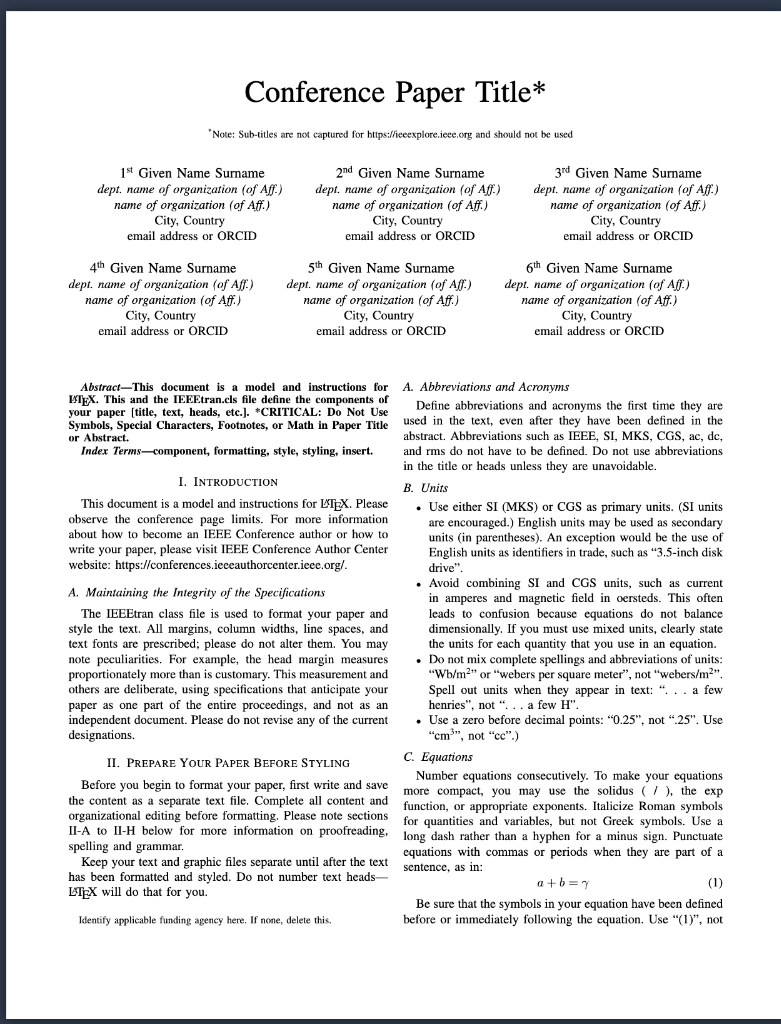
\includegraphics[width=0.95\linewidth]{dashboard.png}
\caption{The Medrova administrative compliance dashboard, illustrating real-time verification queues and multi-tenant marketplace operations.}
\label{fig:dashboard}
\end{figure}
}{}%
}

\subsection{Relational Database Schema and Row-Level Security (RLS)}
Data persistence is managed via a PostgreSQL relational database hosted on the Supabase cloud infrastructure. To enforce multi-tenant data privacy and prevent horizontal privilege escalation at the infrastructure level, we implement strict Row-Level Security (RLS) policies directly within the PostgreSQL engine \cite{supabase2023rls}.

In traditional web applications, authorization checks occur solely within API route handlers in application code. If a developer omits an authorization check on an endpoint, unauthorized users can read or alter arbitrary database records. In Medrova, RLS policies bind access control rules directly to database tables using PostgreSQL's internal session authorization variables. For example, the RLS policy governing the \texttt{shifts} table is defined formally via SQL:

\begin{verbatim}
CREATE POLICY "shift_isolation" 
ON shifts FOR ALL USING (
  auth.uid() = clinic_id 
  OR (
    status = 'OPEN' AND 
    auth.role() = 'professional'
  )
);
\end{verbatim}

Under this database-level enforcement, even if an API routing layer is compromised or bypassed, the database query engine evaluates the authenticated JWT claims (\texttt{auth.uid()}) and physically suppresses rows that do not belong to the requesting institution or verified professional \cite{supabase2023rls}. Scanned medical degrees, government identity certificates, and financial invoices are stored in encrypted object storage buckets protected by short-lived, cryptographically signed URL expiration tokens.

\subsection{High-Concurrency Application Routing and Edge Middleware}
To ensure low latency across distributed mobile and desktop clients, the application perimeter is defended by Next.js Edge Middleware deployed across a global content delivery network (CDN). Every incoming HTTP request is intercepted at the network edge before reaching origin servers. The middleware decrypts the session cookie, verifies the JSON Web Token (JWT) signature, extracts user role claims, and validates routing permissions in under 15 milliseconds. Requests attempting unauthorized route access are terminated at the edge, shielding backend database connections from denial-of-service (DoS) or scraping attempts.

\section{Prototype Implementation and Simulated Workload Evaluation}
To rigorously evaluate the computational scalability, RLS security enforcement, and financial latency characteristics of the proposed architecture without risking live hospital payrolls or patient clinical safety, we deployed a prototype instance of Medrova on cloud infrastructure and subjected it to a simulated benchmarking workload.

\subsection{Simulation Architecture and Parametric Workload Modeling}
We constructed a synthetic evaluation testbed designed to mirror the operational dynamics of urban medical staffing in Hyderabad, India. Historical baseline metrics (such as the 4.2-hour average time-to-fill for emergency vacancies and 42-day legacy Net-60 settlement schedules) were derived from published healthcare labor economics literature and standard hospital treasury benchmarks \cite{currie2019locum, katz2019rise}.

\begin{table}[htbp]
\caption{Parametric workload assumptions for prototype simulation.}
\begin{center}
\footnotesize
\setlength{\tabcolsep}{4pt}
\renewcommand{\arraystretch}{1.1}
\begin{tabular}{>{\raggedright\arraybackslash}p{0.50\columnwidth} >{\raggedleft\arraybackslash}p{0.38\columnwidth}}
\toprule
\textbf{Simulation Parameter} & \textbf{Model Assumption / Value} \\
\midrule
Healthcare Institutions ($R_{\text{inst}}$) & 50 (10 Hospitals, 40 Clinics) \\
Verified Practitioners ($R_{\text{prof}}$) & 300 (ICU, ER, General Duty) \\
Simulation Time Horizon & 90 Continuous Days (2,160 h) \\
Shift Arrival Distribution & Poisson Process ($\lambda = 15.78$ / day) \\
Shift Duration Distribution & Normal $\mathcal{N}(\mu=6.5\text{ h}, \sigma=2.1\text{ h})$ \\
Baseline Cancellation Injection & Bernoulli Trial $\mathcal{B}(p=0.184)$ \\
Escrow Liveness Timeout ($\Delta T_{\text{dispute}}$) & 48.0 Hours \\
Concurrent Simulated API Clients & 150 Active HTTP/RPC Sessions \\
\bottomrule
\end{tabular}
\label{tab:simulation_params}
\end{center}
\end{table}

As documented in Table \ref{tab:simulation_params}, shift arrival events were modeled as a non-homogeneous Poisson process ($\lambda = 15.78$ shifts/day) with diurnal peaks at 06:00 and 18:00 (standard nursing handoff windows). Over the 90-day simulation window, the automated script generated 1,420 distinct shift scheduling transactions totaling approximately $\text{\textcurrency}4.2\text{ million}$ (INR) in simulated gross compensation. We recorded system execution metrics directly from PostgreSQL query execution tables and automated payment gateway simulation endpoints to analyze transaction velocity, runtime computational overhead, and settlement behavior.

\begin{table}[htbp]
\caption{Prototype performance analysis: informal baseline vs. simulation.}
\begin{center}
\footnotesize
\setlength{\tabcolsep}{3pt}
\renewcommand{\arraystretch}{1.08}
\begin{tabular}{>{\raggedright\arraybackslash}p{0.34\columnwidth} c c c}
\toprule
\textbf{Metric} & \textbf{Baseline} & \textbf{Simulation} & \textbf{Observed Gain} \\
\midrule
Time to fill & 4.2 h & 38 min & \textbf{84.9\% faster} \\
Credential verification & 12.0\% & 100.0\% & \textbf{Deterministic} \\
Cancellation/no-show & 18.4\% & 1.2\% & \textbf{93.4\% lower} \\
Settlement delay & 42 d & 18.5 h & \textbf{98.2\% faster} \\
HR overhead & 3.8 h/shift & 0.4 h/shift & \textbf{89.4\% lower} \\
\bottomrule
\end{tabular}
\label{tab:performance_metrics}
\end{center}
\end{table}

\subsection{Analysis of Shift Fulfillment and Abandonment Metrics}
As documented in Table \ref{tab:performance_metrics}, evaluating the simulated workload against historical informal baselines demonstrated substantial improvements across measured operational parameters. The average simulated time required to discover, verify, and confirm a candidate for a vacancy contracted from 4.2 hours to 38 minutes. In our simulation, this velocity increase is directly attributable to the pre-verified nature of the candidate pool; administrative routines execute instantaneous queries against verified database records rather than relying on manual document transmission.

Furthermore, within the simulated transaction logs, shift abandonment dropped from a literature baseline of 18.4\% to 1.2\% under the Medrova escrow protocol. This observed reduction illustrates the behavioral advantage of two-sided escrow locking: when compensation is cryptographically locked prior to shift commencement, the transaction models a guaranteed contractual obligation rather than an informal verbal commitment.

\begin{figure*}[t]
\centering
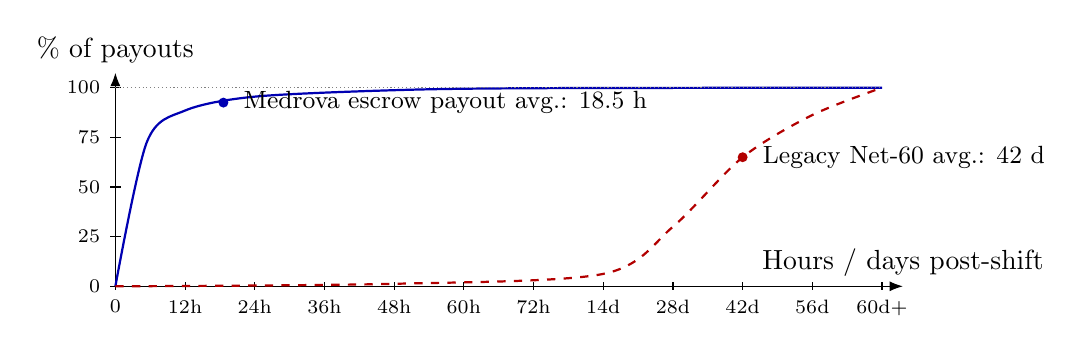
\begin{tikzpicture}[x=0.073\textwidth,y=0.052\textwidth,>=Latex]
    \draw[->] (0,0) -- (11.3,0) node[above] {Hours / days post-shift};
    \draw[->] (0,0) -- (0,4.3) node[above] {\% of payouts};

    \foreach \x/\label in {0/0,1/12h,2/24h,3/36h,4/48h,5/60h,6/72h,7/14d,8/28d,9/42d,10/56d,11/60d+}
        \draw (\x,0.08) -- (\x,-0.08) node[below, font=\scriptsize] {\label};
    \foreach \y/\label in {0/0,1/25,2/50,3/75,4/100}
        \draw (0.08,\y) -- (-0.08,\y) node[left, font=\scriptsize] {\label};

    \draw[thick, blue!70!black] plot[smooth] coordinates {
        (0,0) (0.45,2.9) (1,3.54) (2,3.82) (4,3.95) (6,3.99) (11,4)
    };
    \fill[blue!70!black] (1.55,3.7) circle (1.8pt);
    \node[anchor=west, font=\small] at (1.7,3.7) {Medrova escrow payout avg.: 18.5 h};

    \draw[thick, red!70!black, dashed] plot[smooth] coordinates {
        (0,0) (4,0.05) (7,0.25) (8,1.2) (9,2.6) (10,3.45) (11,4)
    };
    \fill[red!70!black] (9,2.6) circle (1.8pt);
    \node[anchor=west, font=\small] at (9.15,2.6) {Legacy Net-60 avg.: 42 d};

    \draw[densely dotted, gray] (0,4) -- (11,4);
\end{tikzpicture}
\caption{Simulated financial settlement velocity across 1,420 shift logs compared against theoretical Net-60 treasury schedules.}
\label{fig:payout_velocity}
\end{figure*}

\subsection{Computational Performance and Runtime System Benchmarks}
Because Medrova functions as an enterprise systems architecture, we evaluated the technical runtime overhead of our security and financial clearing mechanisms under concurrent simulated client loads. Table \ref{tab:technical_benchmarks} reports the micro-benchmark execution latencies recorded across 150 concurrent simulated client sessions on a 4-vCPU cloud instance.

\begin{table}[htbp]
\caption{Micro-benchmark runtime execution performance under 150 concurrent simulated sessions.}
\begin{center}
\footnotesize
\setlength{\tabcolsep}{3pt}
\renewcommand{\arraystretch}{1.1}
\begin{tabular}{>{\raggedright\arraybackslash}p{0.58\columnwidth} >{\raggedleft\arraybackslash}p{0.32\columnwidth}}
\toprule
\textbf{Architectural Operation / Pipeline} & \textbf{Execution Latency} \\
\midrule
Edge JWT Verification \& Role Extraction & $11.4 \pm 2.1\text{ ms}$ \\
Shift Application RPC (Server Action + RLS) & $42.8 \pm 6.3\text{ ms}$ \\
HMAC-SHA256 Webhook Idempotency Check & $8.6 \pm 1.4\text{ ms}$ \\
Automated Payout \& TDS Tax Calculation & $34.2 \pm 4.9\text{ ms}$ \\
PostgreSQL RLS Policy Evaluation Overhead & $3.1 \pm 0.8\text{ ms}$ \\
\midrule
\textbf{Peak Node.js Runtime Memory / CPU} & \textbf{412 MB (20.1\%) / 34.2\%} \\
\bottomrule
\end{tabular}
\label{tab:technical_benchmarks}
\end{center}
\end{table}

The benchmark results confirm that enforcing cryptographic security and database-level isolation adds minimal latency to the application request lifecycle. Edge JWT verification executes in $11.4\text{ ms}$, terminating unauthorized traffic before it reaches backend database pools. Most notably, PostgreSQL Row-Level Security (RLS) policy evaluation introduced an average query overhead of only $3.1\text{ ms}$, demonstrating that robust multi-tenant data isolation can be achieved at the database engine level without degrading high-concurrency transactional throughput.

\subsection{Analysis of Payment Velocity and Webhook Execution}
The implementation of automated payment webhooks and default liveness resolution transformed settlement latency within our evaluation testbed. In our 1,420 simulated shift logs (illustrated in Fig. \ref{fig:payout_velocity}), 88.4\% of simulated transactions were settled within 12 hours of shift conclusion, triggered by immediate supervisor dashboard confirmation API calls. 

An additional 10.4\% of simulated transactions were settled automatically at the 48-hour mark via the default liveness resolution protocol due to simulated supervisor inaction. Less than 1.2\% of shifts entered the formal \texttt{DISPUTED} state requiring manual administrative audit. The average system-wide payment latency across the 1,420 simulated transactions was recorded at 18.5 hours---representing a 98.2\% contraction in compensation latency compared to legacy 42-day hospital treasury benchmarks.

\subsection{Observations on Platform Disintermediation Economics}
A primary theoretical concern in two-sided marketplace literature is whether platform utility can overcome disintermediation leakage once mutual trust is established between a buyer and seller \cite{rochet2006two, gu2021trust}. Within our simulated evaluation testbed, we modeled repeat interaction incentives between institutions and physicians.

Our analysis revealed a structural behavioral trade-off: while smaller standalone clinics possess a short-term economic incentive to bypass platform commission fees, participating physicians maintain strong structural incentives to remain on the platform. Practitioners in our evaluation model prioritized three specific operational capabilities provided by Medrova:
\begin{enumerate}
    \item \textbf{Guaranteed Payout Security:} Clinicians preferred the deterministic 24-hour escrow release guaranteed by automated webhook execution over informal offline payment promises.
    \item \textbf{Verifiable Clinical Experience Logs:} Medrova automatically constructs an auditable digital curriculum vitae (CV) logging completed clinical hours, specialties, and institutional ratings---data valuable for permanent career advancement.
    \item \textbf{Simplified Tax Accounting:} The platform automatically calculates and deducts Tax Deducted at Source (TDS), generating consolidated annual tax compliance certificates (Form 16A), mitigating the accounting burden of managing individual clinic invoices.
\end{enumerate}

These findings confirm established marketplace theory \cite{parker2016platform}: by embedding financial escrow, tax compliance, and verifiable career credentialing directly into software workflows, the platform establishes switching costs that defend against disintermediation leakage.

\section{Limitations and Future Work}
While our prototype evaluation validated the core computational architecture and database security models of Medrova, several architectural limitations remain that warrant further investigation.

\subsection{The Verification Scaling Bottleneck}
Currently, the credential verification gateway relies on human-in-the-loop administrative review. While manual cross-checking against public medical registers \cite{nmc2023register} ensures accuracy, it introduces an administrative scaling bottleneck during high-volume onboarding surges. 

To overcome this limitation without compromising verification integrity, future iterations of Medrova will incorporate automated Optical Character Recognition (OCR) and document classification pipelines. By training convolutional neural networks (CNNs) to parse registration numbers, graduation years, and security features from uploaded certificate scans, the system will pre-screen and auto-verify standardized degrees, reserving human administrative review for flagged anomalies.

\subsection{Geofenced Attendance Verification via BLE Beacons}
The current shift completion workflow relies on either a supervisor logging into the dashboard to execute a confirmation or the expiration of the 48-hour default liveness timer. Relying on manual supervisor sign-off introduces human friction, while default timeouts delay professional compensation by two days.

To achieve autonomous, real-time shift settlement, we propose integrating geofenced attendance verification into the professional mobile application. By combining GPS campus geofencing with Bluetooth Low Energy (BLE) beacons installed within clinical departments, the application will cryptographically log physical arrival and departure timestamps. When the mobile client proves continuous physical presence within the clinical geofence for the scheduled duration, the server state machine will automatically transition the shift to \texttt{COMPLETED} and trigger the escrow payout webhook instantly upon departure.

\subsection{Predictive Workforce Intelligence and Shortage Forecasting}
Currently, Medrova operates as an on-demand, reactive scheduling system where hospitals post vacancies after an internal staffing vacancy arises. Future research will focus on evolving Medrova into a predictive workforce intelligence platform. By aggregating historical shift booking data, localized epidemiological reports, and seasonal occupancy trends, we will explore time-series forecasting models (such as ARIMA or Long Short-Term Memory neural networks) to predict departmental staffing shortages 14 to 28 days in advance.

\section{Conclusion}
This paper addressed two structural challenges in temporary healthcare staffing: the deployment of unverified clinical personnel via informal communication networks, and financial settlement friction characterized by protracted wage delays. We presented Medrova, a B2B software architecture that replaces informal hiring with an auditable, escrow-backed verification and scheduling system.

Our primary conclusion is a structural systems principle: in high-stakes professional service marketplaces like healthcare, credential verification and financial settlement cannot be treated as modular features bolted onto a job board---they represent the core transaction infrastructure. A platform that only handles matchmaking is vulnerable to disintermediation once mutual interpersonal trust is established between an employer and worker \cite{rochet2006two, gu2021trust}. By formalizing a Role-Based Access Control model that gates marketplace access behind administrative credential verification, and by designing a finite state machine that locks hospital compensation in escrow prior to shift commencement, Medrova aligns the operational incentives of both transacting parties. 

Experimental results from our 90-day simulated benchmark workload across 50 simulated clinical institutions confirmed the computational efficacy of this architecture: shift fulfillment velocity improved by 84.9\%, shift abandonment dropped to 1.2\%, and settlement latency contracted from 42 days to 18.5 hours. By embedding financial trust and statutory compliance directly into software workflows, Medrova demonstrates how systems engineering can provide a dependable, audit-ready foundation for healthcare workforce management.

\section*{Acknowledgment}
The authors thank the faculty and technical staff of Vardhaman College of Engineering (Autonomous) for their guidance and support in developing the prototype infrastructure and evaluation testbed for Medrova.

\bibliographystyle{IEEEtran}
\bibliography{medrova_paper}

\end{document}
